% Section: Quantum Entanglement Geometric Interpretation
\section{Geometric Interpretation of Quantum Entanglement}
\label{sec:entanglement_geometry}

\subsection{The Mystery of Entanglement}

Quantum entanglement—the ``spooky action at a distance''—has been a foundational mystery since the EPR paradox. Standard quantum mechanics describes entanglement algebraically through state vectors, but offers no geometric picture of how correlations occur instantaneously over arbitrary distances.

\begin{insight}[Entanglement as Shared Internal Time]
In UFT, entangled particles share the same \textbf{internal time coordinate} $t_{int}$ while maintaining distinct external (reciprocal) time coordinates $t_{rec}$. This explains instantaneous correlation without violating causality.
\end{insight}

\subsection{The Geometric Framework}

\subsubsection{Two-Particle Entangled State}

Consider two particles $A$ and $B$ in the Bell state:
\begin{equation}
    |\psi_{AB}\rangle = \frac{1}{\sqrt{2}}(|0_A 1_B\rangle - |1_A 0_B\rangle)
\end{equation}

In UFT, this corresponds to:

\begin{equation}
    t_{int}^A = t_{int}^B = t_{int}^{(shared)}
    \quad \text{while} \quad
    t_{rec}^A \neq t_{rec}^B
\end{equation}

\begin{figure}[htbp]
\centering
\begin{tikzpicture}[
    particle/.style={circle, draw, thick, minimum size=1cm},
    label/.style={font=\small}
]

% Particle A
\node[particle, fill=blue!20] (A) at (-3,0) {$A$};
\node[label, below=0.3cm of A] {$t_{rec}^A$};
\node[label, above=0.3cm of A] {$t_{int}^{shared}$};

% Particle B
\node[particle, fill=red!20] (B) at (3,0) {$B$};
\node[label, below=0.3cm of B] {$t_{rec}^B$};
\node[label, above=0.3cm of B] {$t_{int}^{shared}$};

% Internal space connection
\draw[thick, dashed, <->] (A) -- (B) node[midway, above] {Internal Space} node[midway, below] {$t_{int}$ shared};

% External time labels
\node at (-3,-1.5) {External time: $t_{rec}^A$};
\node at (3,-1.5) {External time: $t_{rec}^B$};

% Distance
\draw[<->] (-3,-2) -- (3,-2) node[midway, below] {Spatial separation $d$};

\end{tikzpicture}
\caption{Geometric interpretation of entanglement. Two particles share the same internal time coordinate while having distinct external times and spatial positions.}
\label{fig:entanglement_geometry}
\end{figure}

\subsubsection{Why No Signaling?}

The no-signaling theorem is naturally explained:

\begin{enumerate}
    \item \textbf{Internal time correlation}: Instantaneous (same $t_{int}$)
    \item \textbf{External time evolution}: Local and causal (different $t_{rec}$)
    \item \textbf{Measurement}: Projects shared $t_{int}$ onto local $t_{rec}$
\end{enumerate}

The correlation exists in the internal space (non-local) but any measurement must occur in reciprocal space (local), preventing faster-than-light communication.

\subsection{Entanglement Entropy as Geometric Volume}

\subsubsection{Entanglement Entropy Formula}

In standard QM, entanglement entropy is:
\begin{equation}
    S_A = -\Tr(\rho_A \ln \rho_A)
\end{equation}

In UFT, this becomes a geometric measure:

\begin{theorem}[Entanglement Entropy Geometric Formula]
The entanglement entropy between regions $A$ and $B$ equals the volume of their shared internal space:
\begin{equation}
    S_{AB} = k_B \cdot \frac{\text{Vol}(\mathcal{I}_{AB})}{\text{Vol}(\mathcal{I}_{unit})} \cdot \ln d_{int}
\end{equation}
where $\mathcal{I}_{AB}$ is the shared internal region, and $d_{int}$ is the internal Hilbert space dimension.
\end{theorem}

\subsubsection{Area Law Emergence}

For a bipartition of space, the shared internal volume scales with the boundary area:

\begin{equation}
    S_{AB} \propto \frac{\text{Area}(\partial A)}{\ell_P^{d_s-2}}
\end{equation}

This explains the ubiquitous area law for entanglement entropy in quantum systems.

\begin{figure}[htbp]
\centering
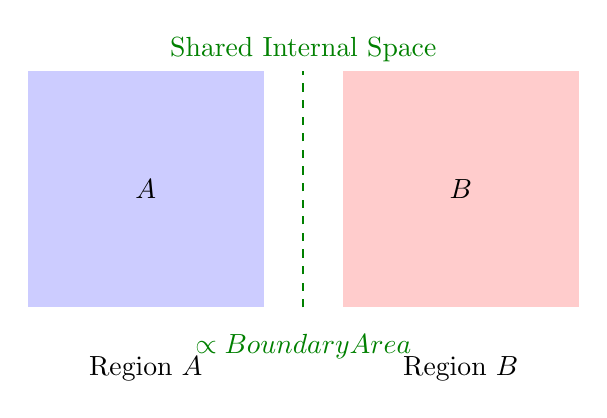
\begin{tikzpicture}

% Region A
\fill[blue!20] (0,0) -- (3,0) -- (3,3) -- (0,3) -- cycle;
\node at (1.5,1.5) {$A$};

% Region B
\fill[red!20] (4,0) -- (7,0) -- (7,3) -- (4,3) -- cycle;
\node at (5.5,1.5) {$B$};

% Boundary (shared internal space)
\draw[thick, dashed, green!50!black] (3.5,0) -- (3.5,3);
\node[green!50!black, above] at (3.5,3) {Shared Internal Space};
\node[green!50!black] at (3.5,-0.5) {$\propto \text{Boundary Area}$};

% Labels
\node[below] at (1.5,-0.5) {Region $A$};
\node[below] at (5.5,-0.5) {Region $B$};

\end{tikzpicture}
\caption{Entanglement entropy scales with the boundary area because the shared internal space ``lives'' at the interface between regions.}
\label{fig:area_law}
\end{figure}

\subsection{Quantum Teleportation as Coordinate Transfer}

\subsubsection{Teleportation Protocol Geometrically}

Standard quantum teleportation transfers an unknown state $|\psi\rangle$ from Alice to Bob using a shared Bell pair and classical communication.

In UFT geometry:

\begin{enumerate}
    \item \textbf{Initial}: Alice has $|\psi\rangle_A$ with $(t_{int}^A, t_{rec}^A)$
    \item \textbf{Entanglement}: Shared Bell pair has $t_{int}^{shared}$ connecting $A$ and $B$
    \item \textbf{Measurement}: Projects $|\psi\rangle$ onto $t_{int}^{shared}$
    \item \textbf{Classical communication}: Transfers $t_{rec}$ information (2 bits)
    \item \textbf{Result}: Bob's particle now has $t_{int}^B = t_{int}^{shared}$ encoding $|\psi\rangle$
\end{enumerate}

\begin{equation}
    \text{Teleportation} = \text{Transfer of } t_{int} \text{ coordinate via shared internal space}
\end{equation}

\subsubsection{Why 2 Classical Bits?}

The 2 bits of classical communication correspond to the projection onto the Bell basis:

\begin{equation}
    |\Phi^+\rangle, |\Phi^-\rangle, |\Psi^+\rangle, |\Psi^-\rangle \rightarrow \text{2 bits of information}
\end{equation}

Geometrically, this is specifying which ``direction'' in the internal space the state occupies.

\subsection{Multipartite Entanglement and Higher Dimensions}

\subsubsection{GHZ States}

For $N$-particle GHZ states:
\begin{equation}
    |GHZ_N\rangle = \frac{1}{\sqrt{2}}(|0\rangle^{\otimes N} + |1\rangle^{\otimes N})
\end{equation}

All $N$ particles share the same internal time:
\begin{equation}
    t_{int}^{(1)} = t_{int}^{(2)} = \cdots = t_{int}^{(N)} = t_{int}^{(shared)}
\end{equation}

The entanglement entropy scales as:
\begin{equation}
    S_{GHZ} = k_B \ln 2 \quad \text{(independent of $N$ for pure state)}
\end{equation}

\subsubsection{Graph States}

More complex entanglement structures correspond to graph connectivity in internal space:

\begin{equation}
    |G\rangle = \prod_{\langle i,j \rangle \in E} CZ_{ij} |+\rangle^{\otimes N}
\end{equation}

where $CZ_{ij}$ creates internal time sharing between connected nodes.

\subsection{Decoherence as Internal Time Desynchronization}

\subsubsection{Environmental Decoherence}

When a quantum system interacts with its environment:

\begin{equation}
    |\psi\rangle_S \otimes |E_0\rangle \rightarrow \sum_i c_i |\psi_i\rangle_S \otimes |E_i\rangle
\end{equation}

In UFT, this is:

\begin{equation}
    t_{int}^{system} \text{ becomes correlated with } t_{int}^{environment}
\end{equation}

The system loses its pure internal time coordinate, becoming mixed.

\begin{theorem}[Decoherence Time Scale]
The decoherence rate is determined by the rate of internal time diffusion:
\begin{equation}
    \Gamma_{dec} = \frac{\tau_0^2}{\hbar} \cdot \frac{k_B T}{E_c} \cdot \langle V_{int}^2 \rangle
\end{equation}
where $\langle V_{int}^2 \rangle$ is the internal space interaction variance.
\end{theorem}

\subsection{ER=EPR in UFT}

The Maldacena-Susskind conjecture states that entanglement (EPR) is equivalent to wormhole connectivity (ER). UFT provides a geometric realization:

\begin{equation}
    \text{ER bridge} = \text{Shared internal space region}
\end{equation}

\begin{figure}[htbp]
\centering
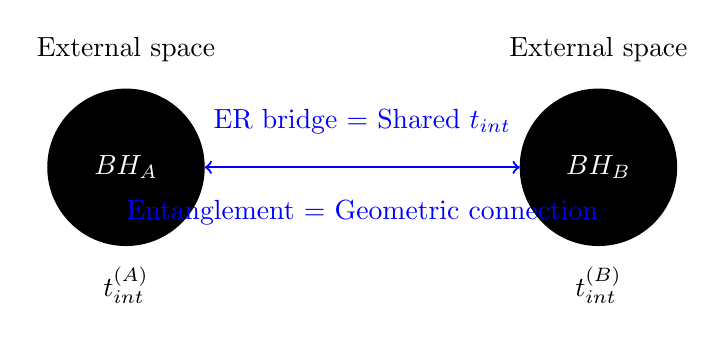
\begin{tikzpicture}

% Black hole A
\fill[black] (-3,0) circle (1cm);
\node[white] at (-3,0) {$BH_A$};
\node at (-3,-1.5) {$t_{int}^{(A)}$};

% Black hole B
\fill[black] (3,0) circle (1cm);
\node[white] at (3,0) {$BH_B$};
\node at (3,-1.5) {$t_{int}^{(B)}$};

% ER bridge (shared internal space)
\draw[thick, blue, <->] (-2,0) -- (2,0);
\node[blue, above] at (0,0.3) {ER bridge = Shared $t_{int}$};
\node[blue, below] at (0,-0.3) {Entanglement = Geometric connection};

% Labels
\node at (-3,1.5) {External space};
\node at (3,1.5) {External space};

\end{tikzpicture}
\caption{ER=EPR in UFT: Entangled black holes are connected by a wormhole (ER bridge) in the internal space, corresponding to shared internal time coordinates.}
\label{fig:er_epr}
\end{figure}

\subsection{Experimental Signatures}

UFT's geometric interpretation makes specific predictions:

\begin{table}[htbp]
\centering
\caption{Testable Predictions for Entanglement Geometry}
\begin{tabular}{@{}lccc@{}}
\toprule
\textbf{Prediction} & \textbf{UFT Value} & \textbf{Standard QM} & \textbf{Testable} \\
\midrule
Max entanglement distance & $\infty$ (internal) & $\infty$ & No \\
Decoherence scaling & $\tau_0^2 T/E_c$ & Environment model & Yes \\
Entanglement sudden death & Never (pure $t_{int}$) & Environment-dependent & Indirect \\
Multipartite scaling & Area law from geometry & Conjectured & Yes \\
\bottomrule
\end{tabular}
\label{tab:entanglement_predictions}
\end{table}

\subsection{Summary}

\begin{insight}[Entanglement Geometry Summary]
Quantum entanglement in UFT:
\begin{itemize}
    \item Is \textbf{shared internal time coordinates} between particles
    \item Explains instantaneous correlation (same $t_{int}$)
    \item Preserves no-signaling (measurement in $t_{rec}$)
    \item Scales entanglement entropy with boundary area
    \item Unifies ER=EPR through geometric wormholes
    \item Treats decoherence as internal time desynchronization
\end{itemize}
\end{insight}

The geometric interpretation transforms entanglement from a mysterious algebraic property into an intuitive spacetime structure: particles are ``connected'' through the internal space, while appearing separate in our observable 4D world.